\chapter{系统实现}
根据上面的调研结果,可以改进的方面有很多。但是从用户日常使用的角度,影响用户持续使用最大的问题是可用性的问题和理解的问题。

可用性的解决方案主要分为两块:一个是提高系统的可用性;另一个是重新设计用户友好的交互界面,提升交互的体验。增强用户理解则是通过加入透明性。

如图\ref{fig:system}所示,系统主要分为两部分:服务端和客户端。

\begin{figure}[ht]
    \centering
    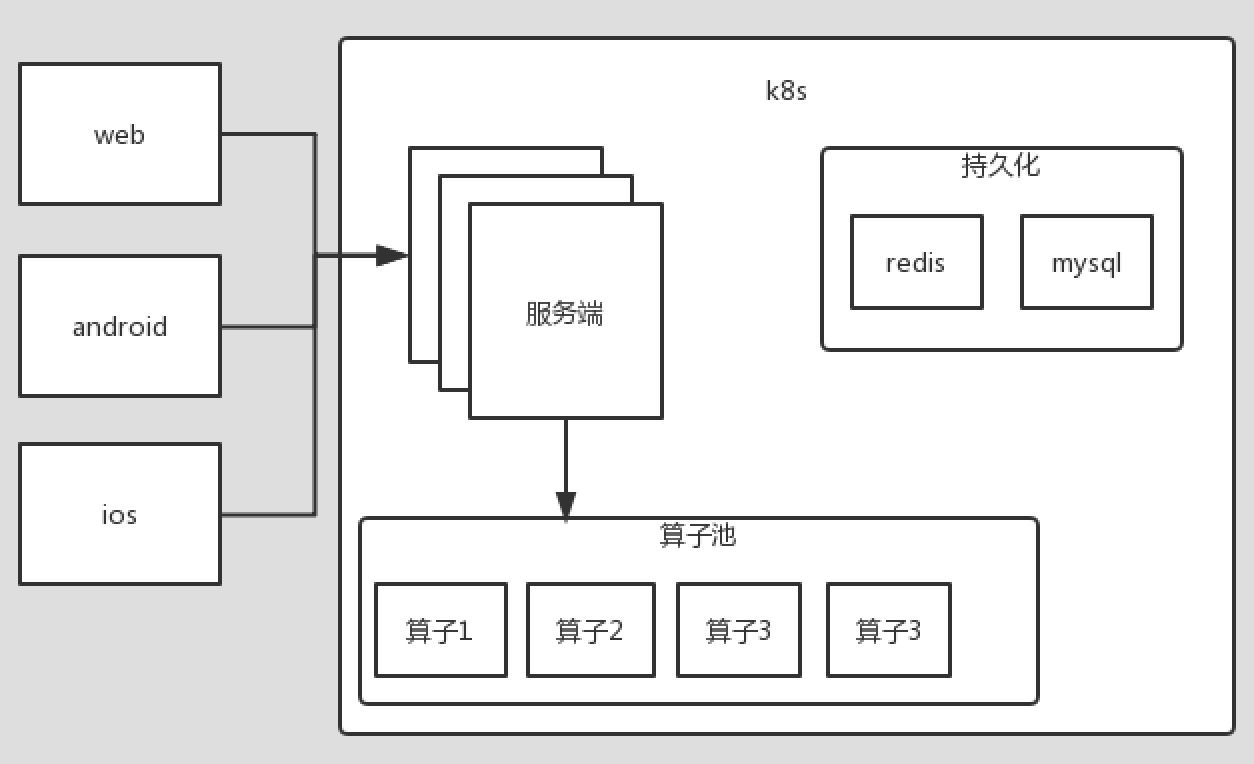
\includegraphics[width=12cm]{images/system.png}
    \caption{系统设计}
    \label{fig:system}
\end{figure}

一次诊断的大致流程如下:用户通过客户端,上传图片或者回答问题,客户端则向服务端发起请求。服务端收到请求之后,进行任务分配,对分配到任务的实例,调用对应的模型完成特征提取或诊断打分,同时将数据持久化到redis和mysql中,然后把结果返回给客户端。客户端收到服务端的结果后,根据用户是否透明,进行结果的展示。

\section{模型池}

为了能够满足系统的跨平台使用,我们需要把特征提取算法从客户端剥离到服务器,通过接口调用的方式来实现面诊和舌诊,同时在服务的实现诊断算法。

首先,我们使用容器的方法,通过flask本地调用的方法,把特征提取模型打包成服务。每个特征提取服务,可以接受http的请求,对传过来的图片进行特征提取。模型的计算能力如\ref{tab:face-feature}, \ref{tab:tongue-feature}, \ref{tab:diag-feature}所示。

模型池中的模型服务目前有两类,特征提取模型(面部和舌部)和诊断打分模型,分别有对图片进行特征提取和对特征进行打分的能力。服务端有多个实例,共同处理用户发起的诊断任务,使用redis和mysql进行数据的持久化。客户端使用mui框架加上angular及其插件完成,复杂计算和逻辑通过后台调用实现。

\begin{table}[]
    \begin{tabular}{llr}
        \toprule
        特征          & 特征描述     & 特征内容 \\ 
        \midrule
        faceDetectRes & 人脸   & 0:未检测出人脸,1:成功检测出人脸  \\
        faceColor     & 面部颜色 & 0:面白,1:面黑,2:面红,3:面黄,4:面青,5:正常 \\
        faceGloss     & 面部光泽 & 0:有光泽,1:少光泽,2:无光泽\\
        lipDetectRes  & 嘴唇   & 0:未检测出嘴唇,1:成功检测出嘴唇\\
        lipColor      & 嘴唇颜色 & 0:淡白,1:淡红,2:红,3:暗红,4:紫   \\
        \bottomrule
    \end{tabular}
    \caption{脸部特征提取算子输出}
    \label{tab:face-feature}
\end{table}


\begin{table}[]
    \begin{tabular}{llr}
        \toprule
        特征 & 特征描述 & 特征内容 \\ 
        \midrule
        tongueDetectRes & 舌体 & 0:未检测出舌像,1:成功检测出舌像 \\
        tongueCrack & 舌裂纹 & 0:未检测到裂纹,1:成功检测到裂纹 \\ 
        tongueFatThin & 舌胖瘦 & 0:正常(瘦),1:胖舌 \\
        tongueCoatThickness & 舌苔厚薄 & 0:薄,1:厚 \\
        tongueCoatColor & 舌苔颜色 & 0:苔白,1:苔黄 \\
        tongueNatureColor & 舌质颜色 & 0:舌暗红,1:舌淡白,2:舌淡红,3:舌红,4:舌紫\\
        \bottomrule
    \end{tabular}
    \caption{舌部特征提取算子输出}
    \label{tab:tongue-feature}
\end{table}


\begin{table}[]
    \begin{tabular}{lll}
        \toprule
        特征 & 特征描述 & 特征内容 \\ 
        \midrule
        healthScore & 健康分数 & 0-100 \\
        healthType & 是否包含某种体质 & {[}0, 0, 0, 0, 0, 0, 0{]} \\ 
        questionScore & 各种问题的体质得分 & {[}0, 0, 0, 0, 0, 0, 0{]} \\
        symCount & 各种体质症状个数 & {[}0, 0, 0, 0, 0, 0, 0{]} \\
        symNum & 总体体质症状个数 & 0-13 \\
        baseScore & 基本分数 & 0-100 \\
        phy & 体质结果 & 八种体质中的一种\\
        \bottomrule
    \end{tabular}
    \caption{诊断打分算子输出}
    \label{tab:diag-feature}
\end{table}


如\ref{tab:diag-feature}所示,最终诊断打分算子的体质结果输出为 "阳虚","阴虚", "痰湿","瘀滞", "脾虚", "肾虚", "气虚", "健康" 中的一种。

模型部署在docker上,通过k8s管理多个模型高实现可用。服务端通过k8s提供的cluster ip进行调用。为了减少读写的竞争,模型服务池不进行mysql和redis的读写,任务异步完成之后,通过回调服务端的方式,由服务端对结果进行持久化。

\section{服务端}

\subsection{日志管理}
为了方便后续的数据分析,我们需要采用用户的所有操作日志。日志的数据库主要字段如下:


\begin{table}[]
    \begin{tabular}{lll}
        \toprule
        字段 & 类型 & 描述 \\ 
        \midrule
        id & int & 主键 \\
        user, & text & 用户唯一标识 \\ 
        device & text & 所用设备信息 \\
        op & text & 操作 \\
        info & text & 操作信息 \\
        createTime & datetime & 创建时间 \\
        updateTime & datetime & 更新时间\\
        \bottomrule
    \end{tabular}
    \caption{操作日志表}
    \label{tab:op_log}
\end{table}


其中,user字段用于标识用户,默认使用用户手机号作为唯一标识,要求用户进入系统前需要通过手机验证码进行登录。而在后续的透明性实验环节,为了方便用户跳转完成问卷,不需要用户进行登录,user字段采用的是wjx-问卷星id。

\subsection{服务端高可用}
为了实现服务的稳定性,服务端支持开启多个实例;同时考虑到性能,服务端设计为读写分离的架构:每个实例都可以读取任务列表,处理用户的任务,但只有master有任务分配的权限。同时,服务端通过心跳包探活,master失效时,通过redis的分布式锁实现master的竞选。
% \begin{figure}
%     \centering
%     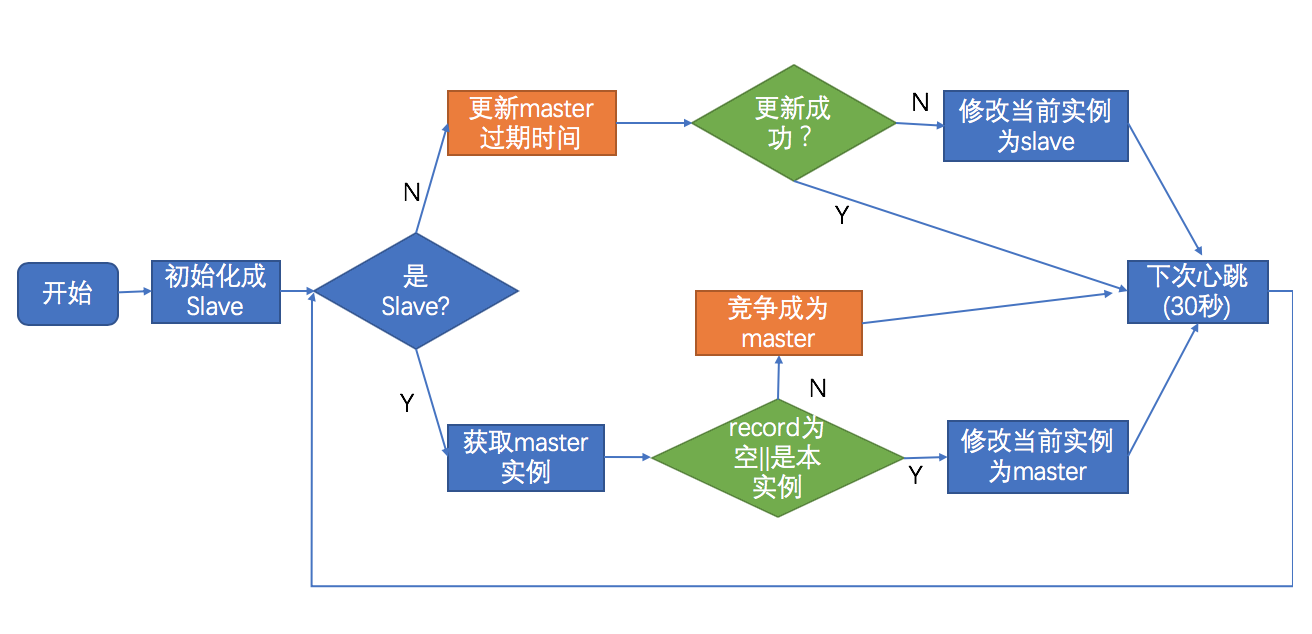
\includegraphics[width=12cm]{images/slave-master.png}
%     \caption{服务端竞选}
%     \label{fig:my_label}
% \end{figure}
通过任务的id进行哈希,按照哈希进行任务的分配。每个服务端实例过一定的间隔时间,就会去读取任务列表,开始执行任务列表里的任务。

\subsection{任务处理}
一次用户诊断,服务端需要完成多个任务:面部特征提取任务,舌部特征提取任务,问诊打分任务。
服务端在收到用户提交的任务之后,会将数据存储到数据库的task表中,task表的主要字段如【TODO】。


\begin{table}[]
    \begin{tabular}{lll}
        \toprule
        字段 & 类型 & 描述 \\ 
        \midrule
        id & int & 主键 \\
        type, & int & 任务类型: 面部,舌部,诊断 \\ 
        in & text & 任务输入 \\
        out & text & 任务结果 \\
        handler & text & 分配的服务端 \\
        status & int & 任务状态: 新建,已分配,处理中,失败,完成 \\
        createTime & datetime & 创建时间 \\
        updateTime & datetime & 更新时间\\
        \bottomrule
    \end{tabular}
    \caption{任务表}
    \label{tab:task}
\end{table}

type一共有三种类型,面部特征提取任务,舌部特征提取任务,和诊断任务。

面部特征提取和舌部特征提取任务需要的输入为图片,通过base64编码序列化为json对象,保存的in字段中。



服务端在获取到分配给自己的任务之后,便会按照任务的类型请求模型池对应的模型完成计算。模型返回结果之后,服务端将结果缓存到redis中,然后写入到mysql数据库中,再返回给客户端。

\section{客户端}
设计新的自诊界面,解决交互方面易用性的问题,给用户对自己当前状态一种直观的感受。
\begin{figure}[ht]
    \centering
    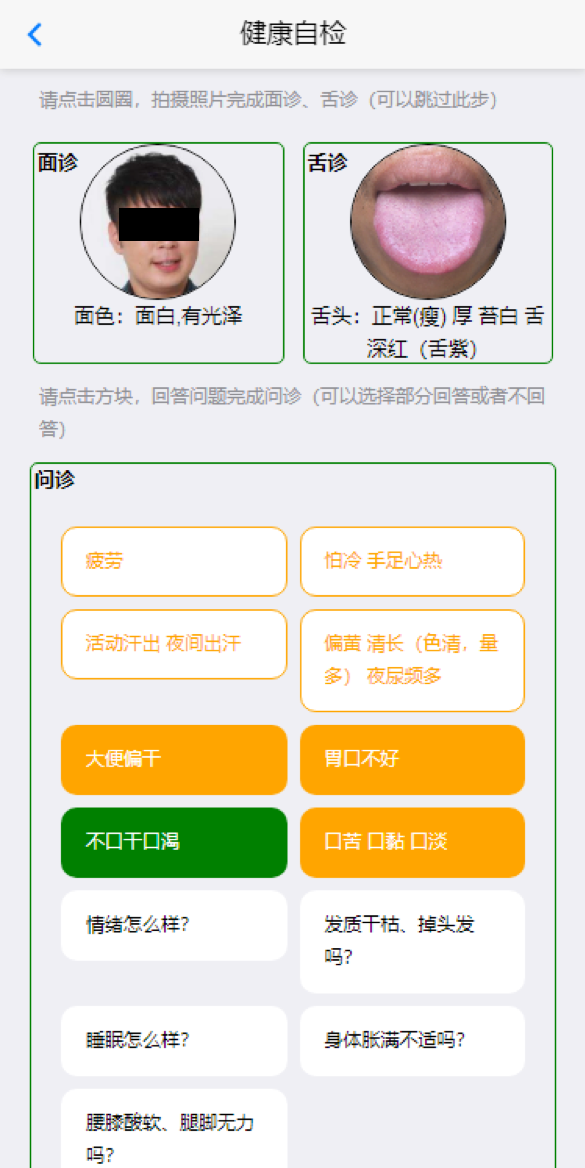
\includegraphics[height=12cm]{images/diag.png}
    \caption{面诊舌诊问诊新界面}
    \label{fig:diag_new}
\end{figure}

如图\ref{fig:diag_new}所示,根据用户调研的反馈,新界面简化了诊断的流程,面诊舌诊问诊在一个页面显示,并且所有的问题和操作都是可选的,不会出现必须要先面诊然后舌诊然后才能问诊的问题。其次,新界面对面诊和舌诊进行了中间结果的反馈,面诊在用户拍照确认之后,会立即报告本次照片是否合格已经诊断的结果,用户不需要在点击诊断的时候才被提示照片不合格。

在问诊方面,新系统实现了最近一次记录保存,由于问题是可选回答的,所以用户只需要回答和自己上次的结果不一致的即可。同时,我们对不同问题的回答结果进行了颜色的区分。有色实心代表本次回答,有色空心代表上次回答;橙色代表有症状,绿色代表回答的问题表现良好,没有症状;白色没有填充和边框,为黑字,代表未回答。

在方框内部的问题描述设计上,我们把默认的文字描述,显示为问题描述;一旦用户本次或者上次回答过该问题,则直接显示用户回答的结果。这样做的结果是,第二次用户点进来,就能看到上次的回答结果,这样能够对自己的身体情况有个快速的了解。

客户端系统主要有以下几个部分:用户登录,健康诊断(面诊,舌诊,问诊),健康报告,诊断记录。

\subsubsection{用户登录}
\begin{figure}[ht]
    \centering
    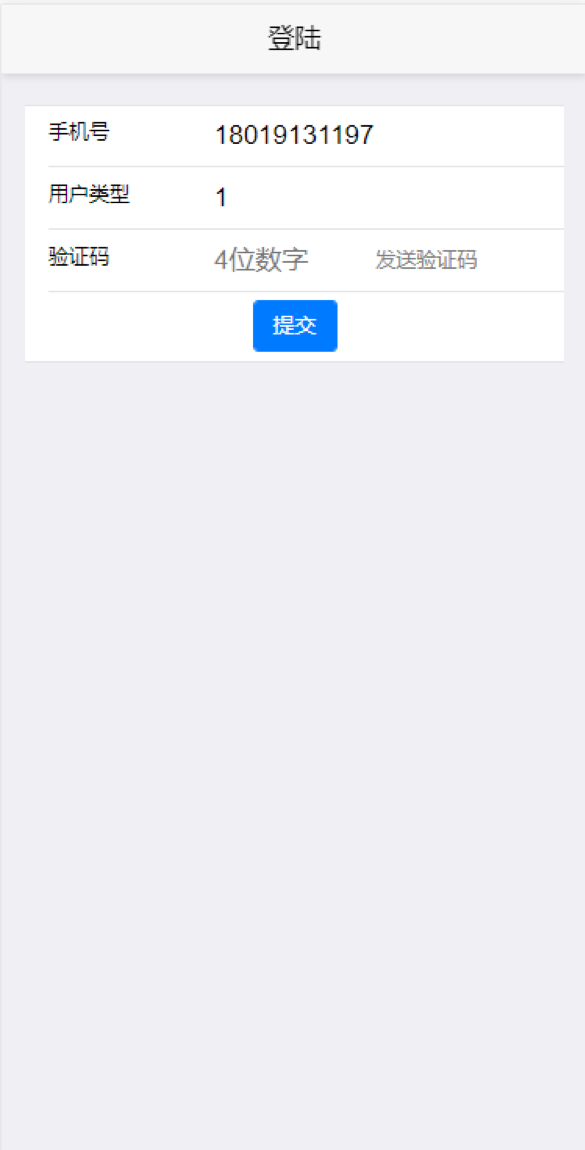
\includegraphics[height=12cm]{images/login.png}
    \caption{用户登录}
    \label{fig:login}
\end{figure} 
用户登录时,需要输入正确的手机号才能通过手机格式验证发送验证码到手机上。登录界面可以接受一个ssojump的参数,用于判断是否来自问卷星。如果验证通过,则直接跳过登录进入首页。
 
% \subsubsection{系统首页}
%  \begin{figure}[h]
%      \centering
%      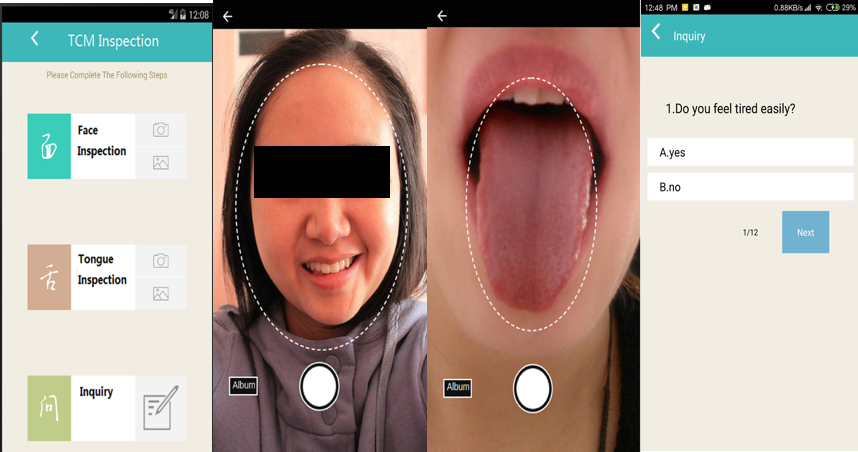
\includegraphics{images/main.png}
%      \caption{Caption}
%      \label{fig:my_label}
%  \end{figure}
% 首页简化之后,只保留了新版和旧版界面的入口,方便用户进行对比,同时,用户也可以在首页下面的tab页查看自己之前的诊断记录。

\subsubsection{健康诊断}

\begin{figure}[ht]
    \centering
    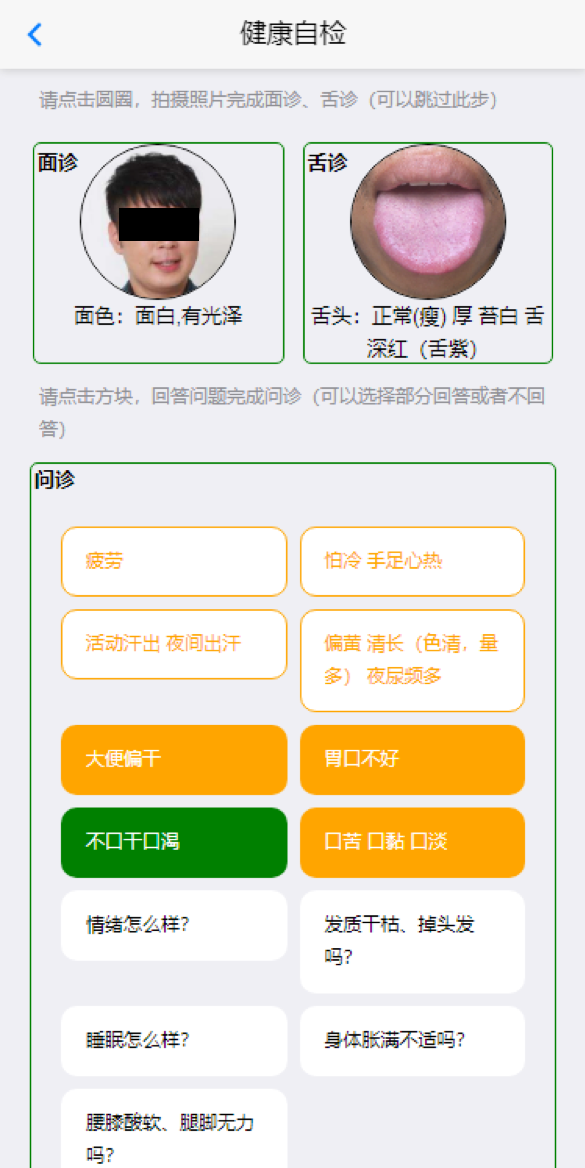
\includegraphics[height=12cm]{images/diag.png}
    \caption{Caption}
    \label{fig:diag}
\end{figure}
新界面和之前版本的云中医界面不同的是,诊断界面不仅提供了面诊舌诊问诊的入口,同时会将面诊舌诊的照片和中间结果直接显示在当前页面,给用户对于自己当前身体情况一个直观的感受。如果拍照失败会直接显示,不需要等到用户进行点击诊断之后才知道自己的照片不合格。
	
\subsubsection{照片上传}

\begin{figure}[ht]
    \centering
    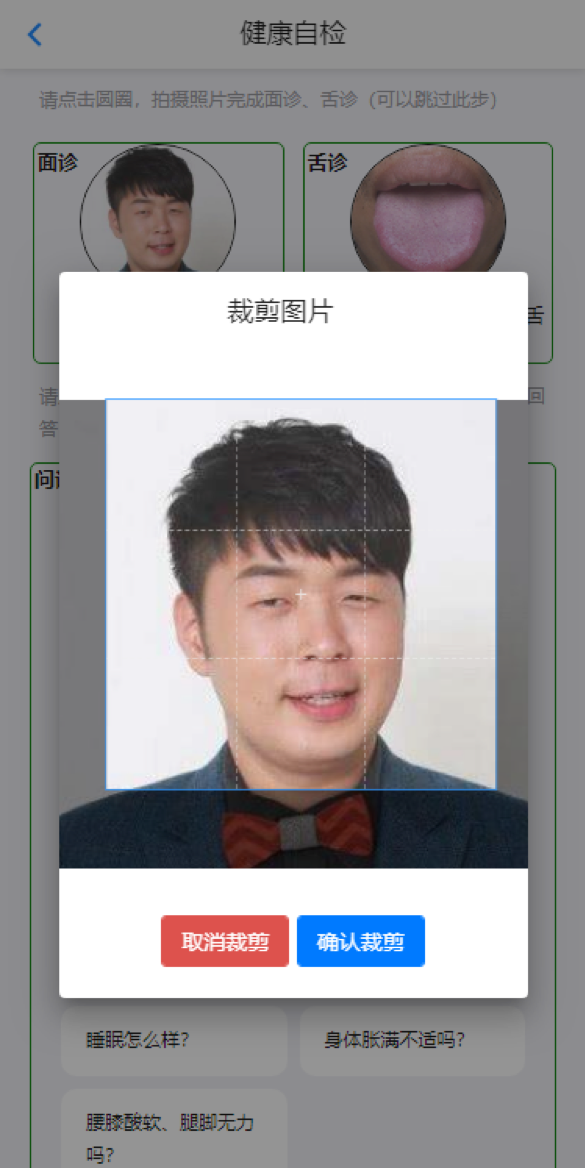
\includegraphics[height=12cm]{images/crop.png}
    \caption{Caption}
    \label{fig:crop}
\end{figure}
用户通过点击面诊或者舌诊的圆圈图案,可以通过从相册选择或者通过拍照,上传自己的脸部或者舌头照片。图片裁剪可以帮助用户定位面部和舌头的位置,提高诊断的精度。用户点击确认裁剪之后,诊断的结果会直接显示在圆圈下面,同时,如果没有识别到人脸或者舌头也会提示用户重新拍照。点击确认裁剪后,通过对图片进行base64编码上传到服务器的诊断接口,服务器调用对应算子,拿到诊断结果。

\subsubsection{问诊}

\begin{figure}[ht]
    \centering
    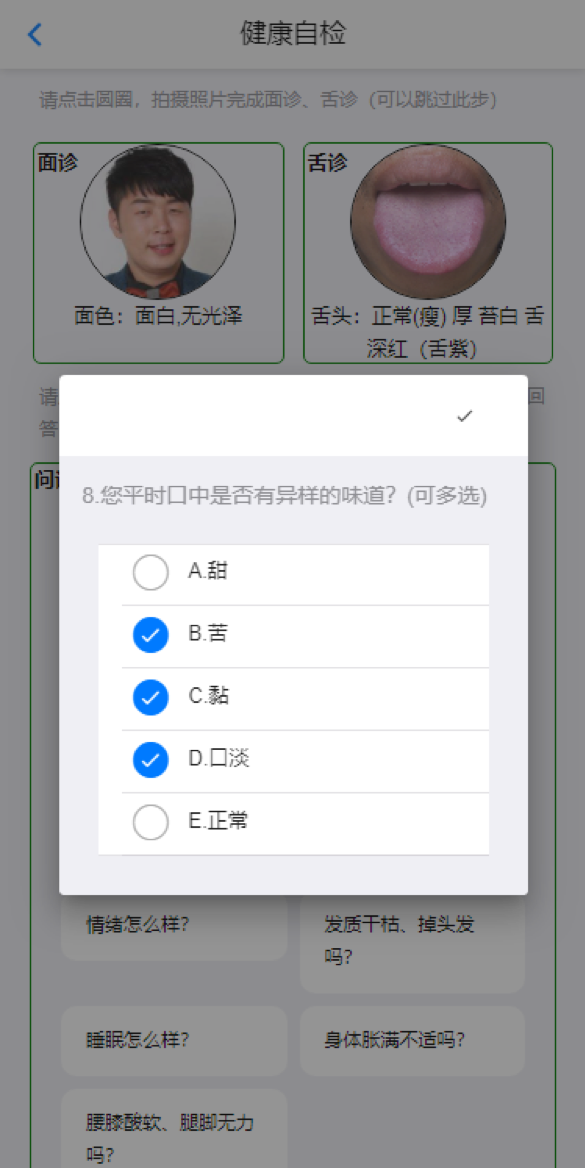
\includegraphics[height=12cm]{images/questions.png}
    \caption{问诊}
    \label{fig:questions}
\end{figure}
问诊的问题一共13道,用户根据自己的情况通过勾选回答问题。每次进入问诊界面,系统会尝试加载上一次用户回答问题的历史记录和对应的答案。同时,回答过的问题,会在界面上进行显示。没有回答过的问题,将是白色黑字没有边框。


用户在完成自己需要回答的问题或者面诊舌诊之后,可以点击蓝色的诊断按钮进行健康诊断,同时,系统会将本地诊断记录上传到后台服务器上,以便查询诊断记录。

\subsubsection{诊断结果}
\begin{figure}[ht]
    \centering
    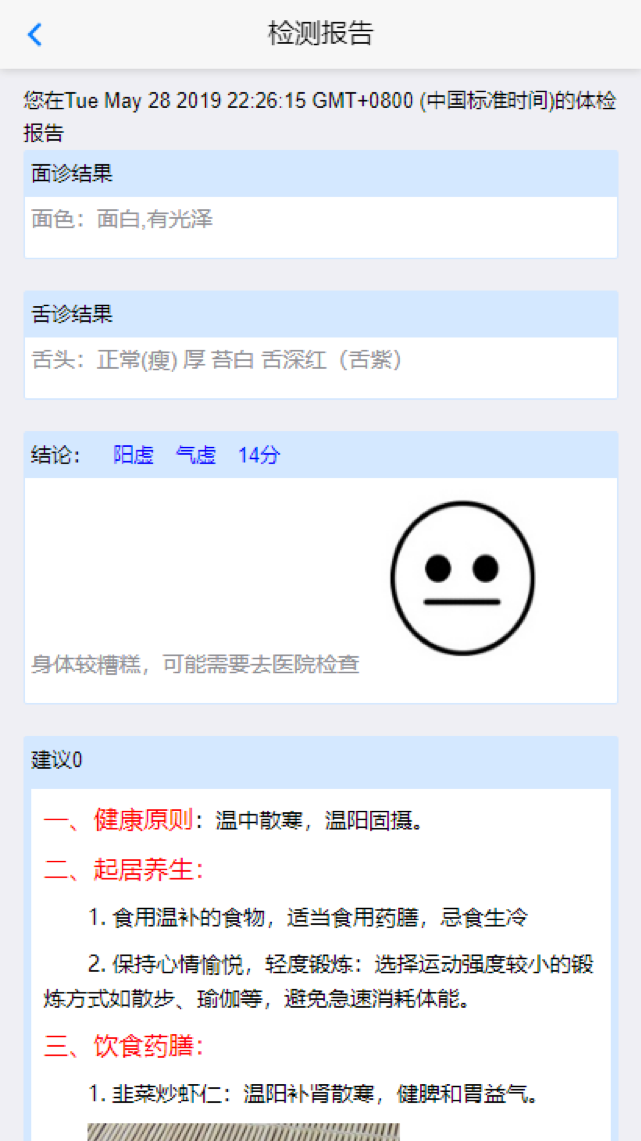
\includegraphics[height=12cm]{images/report.png}
    \caption{健康报告}
    \label{fig:report}
\end{figure}
系统根据用户个人的情况,会给出面诊结果,舌诊结果和最后的体质以及健康分数。此外,根据体质的不同,会给出和体质对应的健康建议,帮助用户进行针对性的健康调理。

\subsubsection{诊断记录列表}
\begin{figure}[ht]
    \centering
    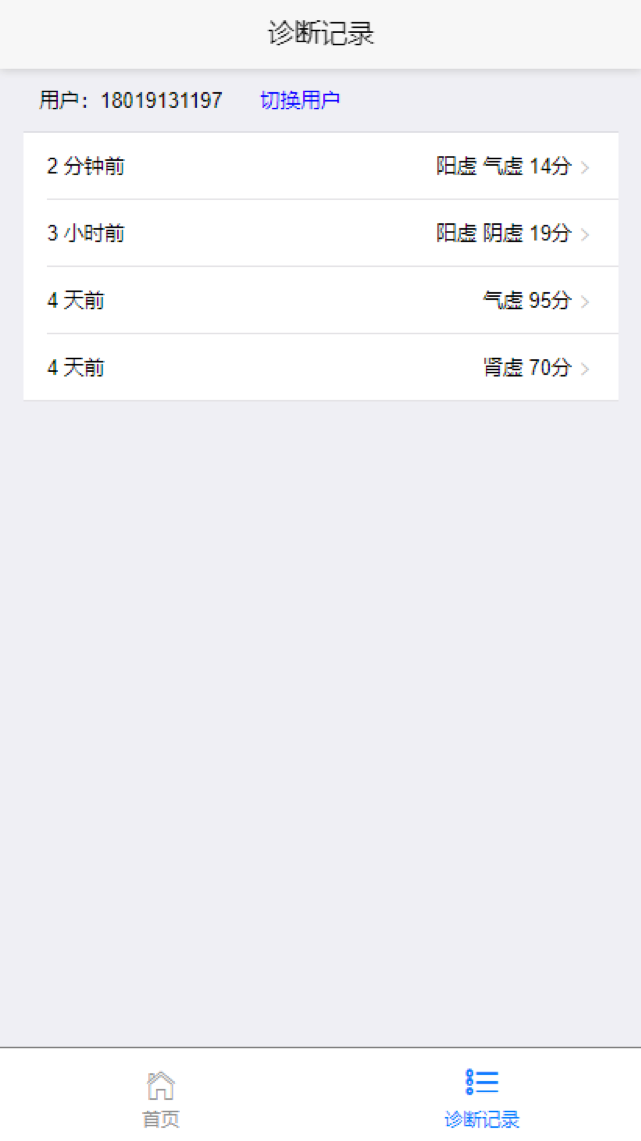
\includegraphics[height=12cm]{images/history.png}
    \caption{诊断历史}
    \label{fig:history}
\end{figure}
诊断记录页面,能够直观地给出用户近期的健康变化的情况。用户可以点击诊断记录,进入当时的详细诊断结果页面。

%%%%%%%%%%%%%%%%%%%%%%%%%%%%%%%%%%%%%
\section{透明性}
考虑到中医应用的特殊性,普通用户需要提高对应用的理解。因此我们在系统中加入算法的透明性,提升用户的体验。

对于每一个用户,我们通过哈希算法,对用户名计算哈希值,按照哈希值的奇偶性,将奇数用户归类为不透明用户,偶数用户归类为透明用户。两类用户在进行面诊舌诊时的流程一样,但是透明用户能够看到背后特征提取算法和诊断算法的中间数据,同时系统为给出的诊断结果进行了解释。

\subsection{面诊舌诊的透明性}
普通用户在面诊页面

\subsection{问诊的透明性}

\subsection{诊断结果的透明性}
\begin{figure}[ht]
    \centering
    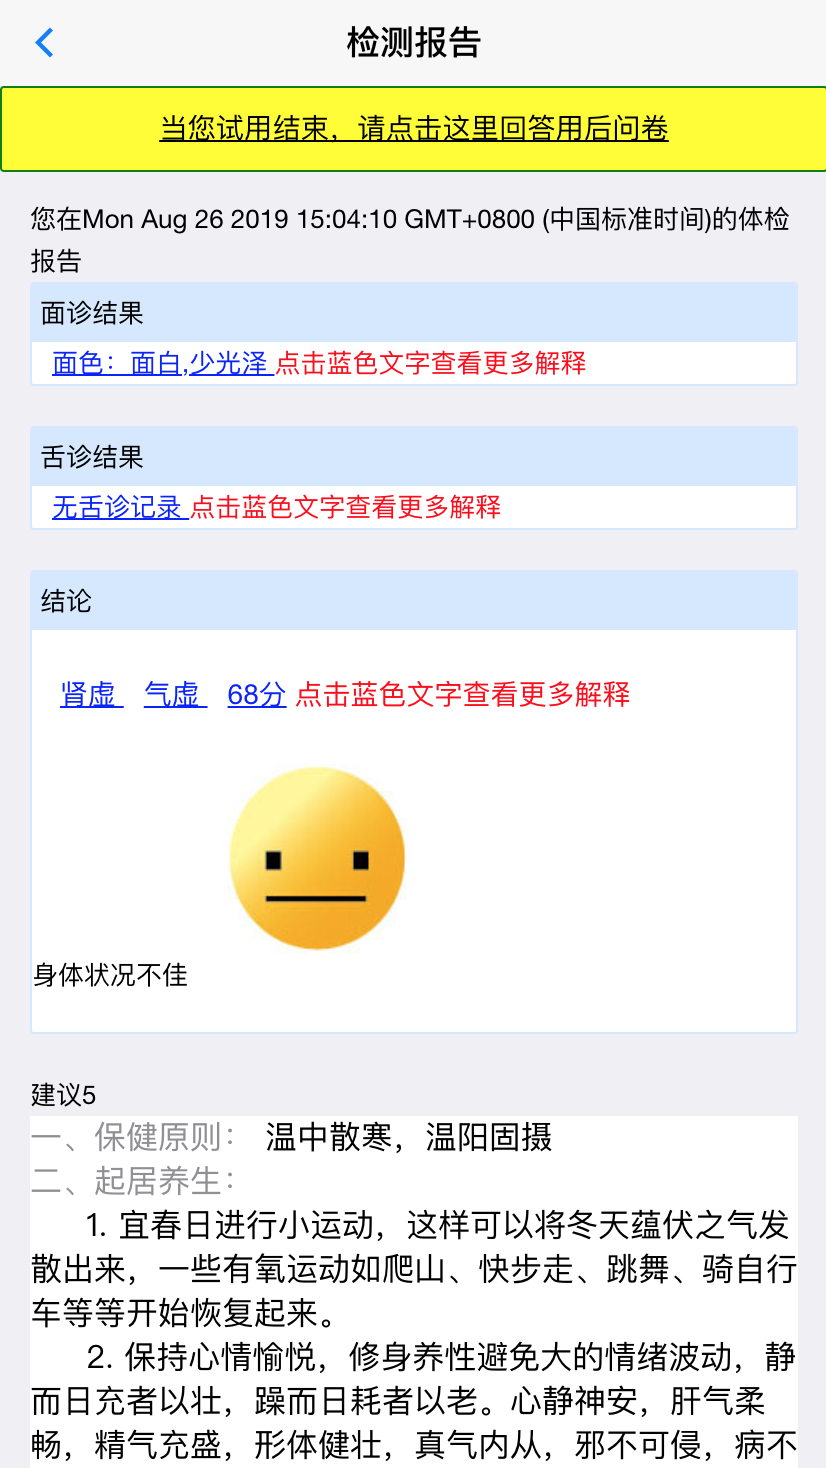
\includegraphics[height=12cm]{images/report3.png}
    \caption{透明用户看到的诊断报告}
    \label{fig:my_label}
\end{figure}

普通用户在诊断结果页面,可以看到自己的健康分数和体质结果;透明用户可以点击诊断分数,了解这个分数是根据哪些指标,通过哪一个算法计算过来的。如图\ref{fig:report_expalin_score}所示,用户点击诊断页面的分数之后,弹窗里会显示分数相关的问题、雷达图和分数计算公式。

分数相关问题,展示了面诊舌诊对体质分数的影响和问诊对体质分数的影响,无影响的问题则不会显示。其中体质分数的变化分两种,一个是分数的累加,另一种是体质分数的清空。

雷达图对体质分数进行了汇总,给用户展示最终个人的体质倾向的结果。

根据诊断打分算子的内部算法,解释页面的计算公式一共有5种类别,我们使用选项卡的方式,将所有的打分计算公式全部透明给用户,并且默认打开当前计算公式的选项卡。

\begin{figure}[ht]
    \centering
    \subfigure[相关问题]{
        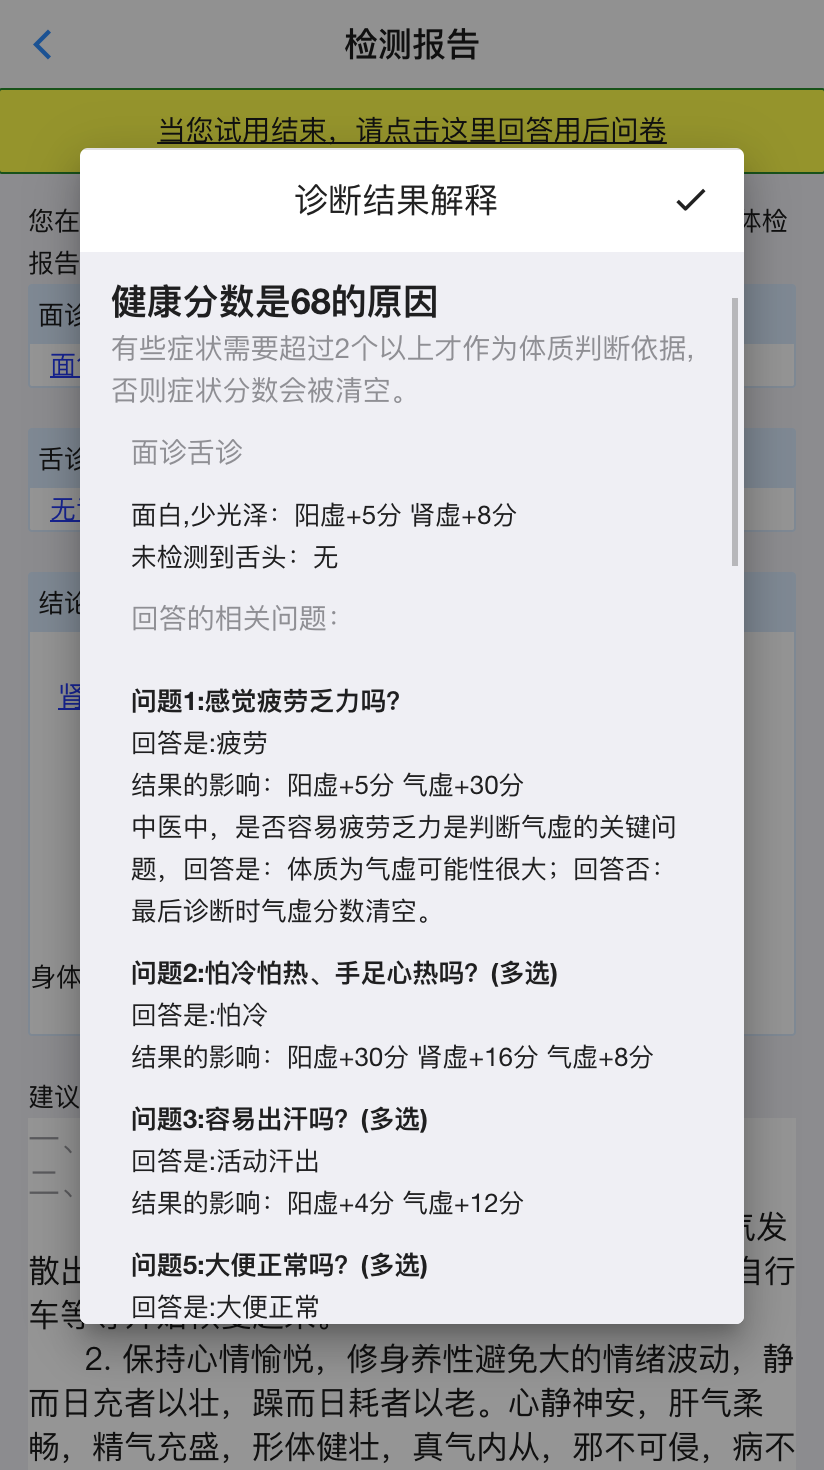
\includegraphics[height=8cm]{images/report7.png}
    }
    \subfigure[雷达图]{
        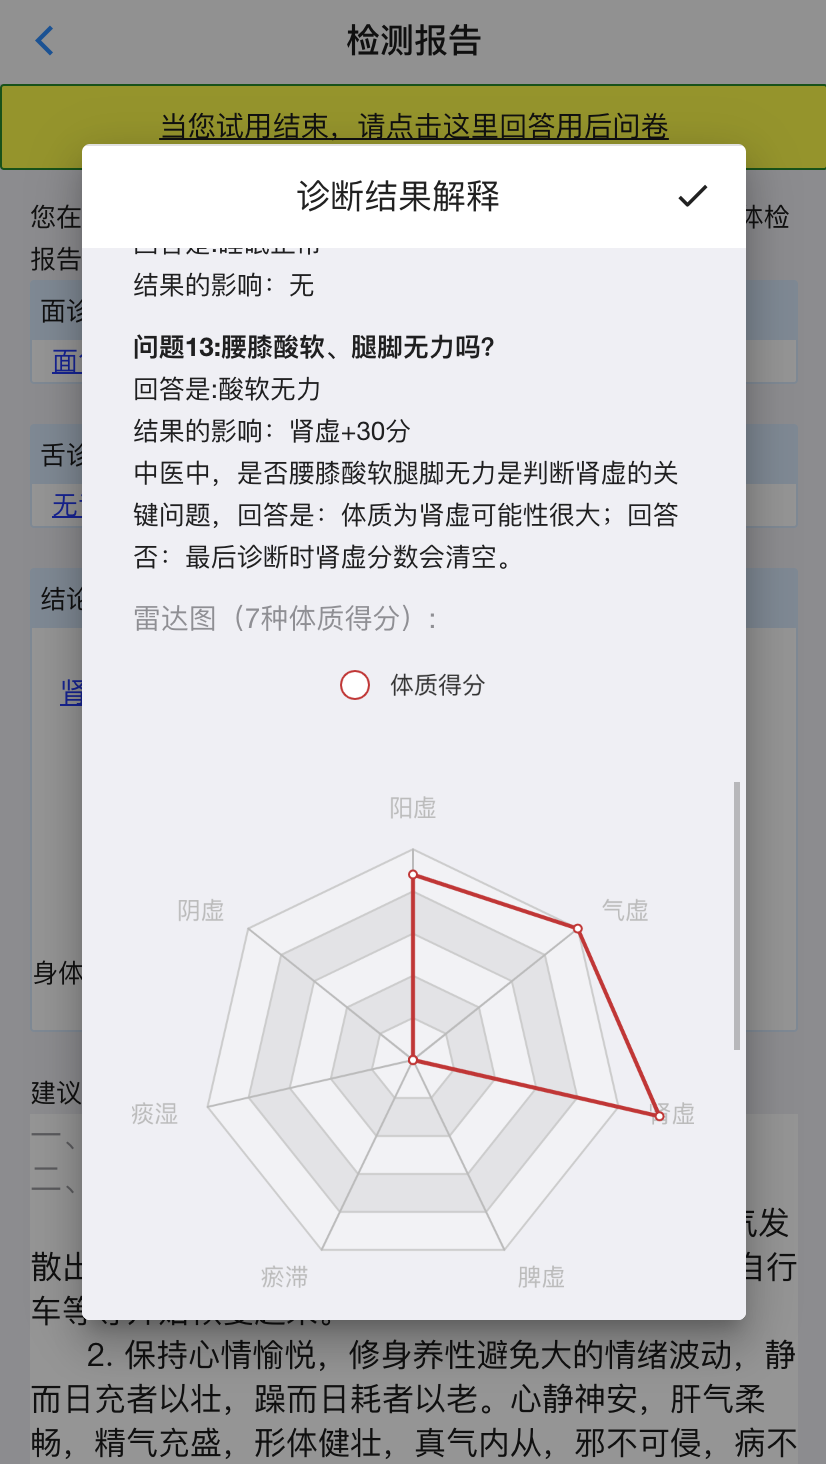
\includegraphics[height=8cm]{images/report8.png}
    }
    \subfigure[计算公式]{
        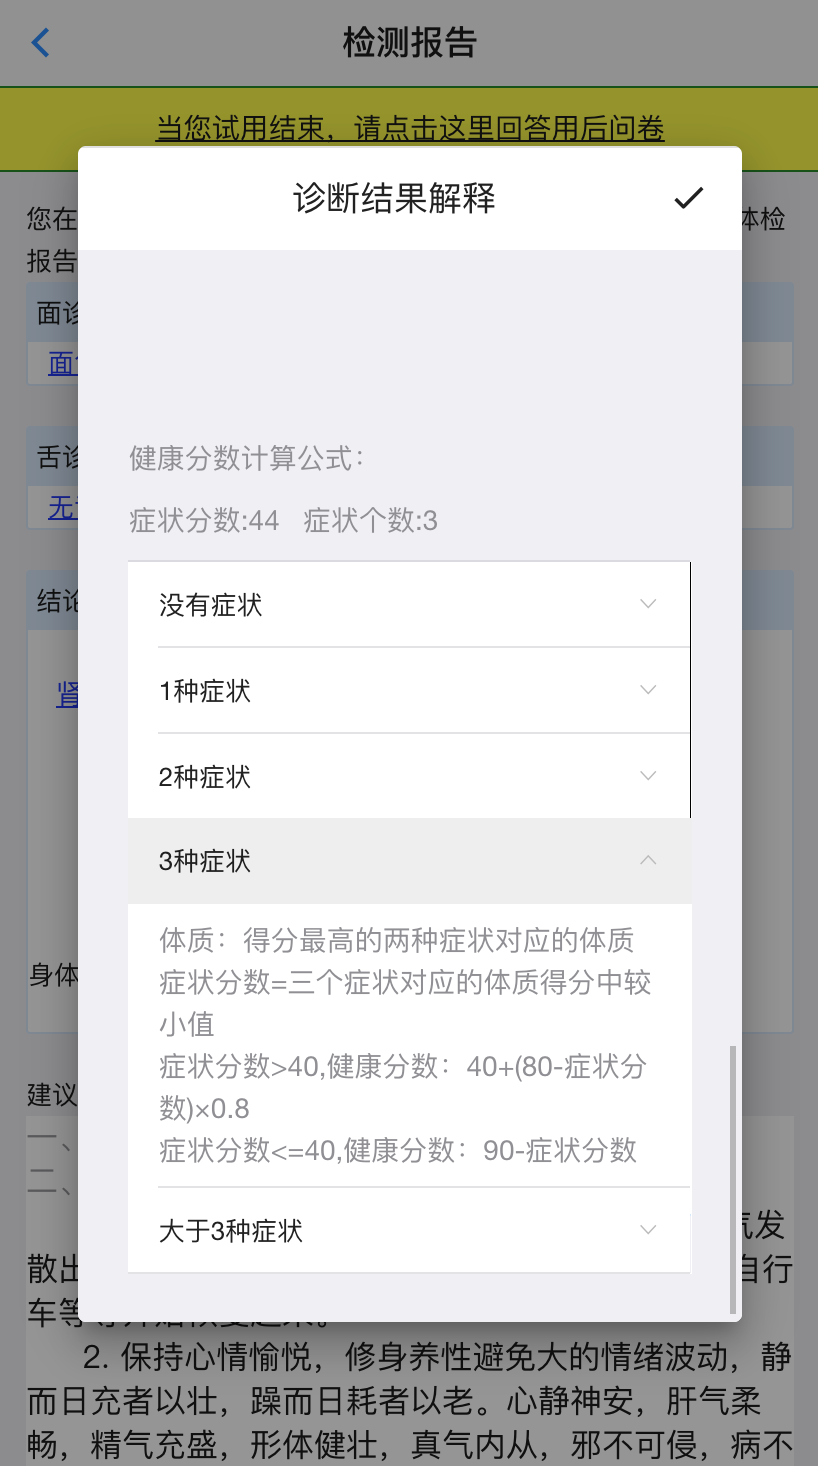
\includegraphics[height=8cm]{images/report9.png}
    }
    \caption{分数的解释}
    \label{fig:report_expalin_score}
\end{figure}

点击面诊结果,可以看到自己的面部舌部的对于整个诊断的影响。
\begin{figure}[ht]
    \centering
    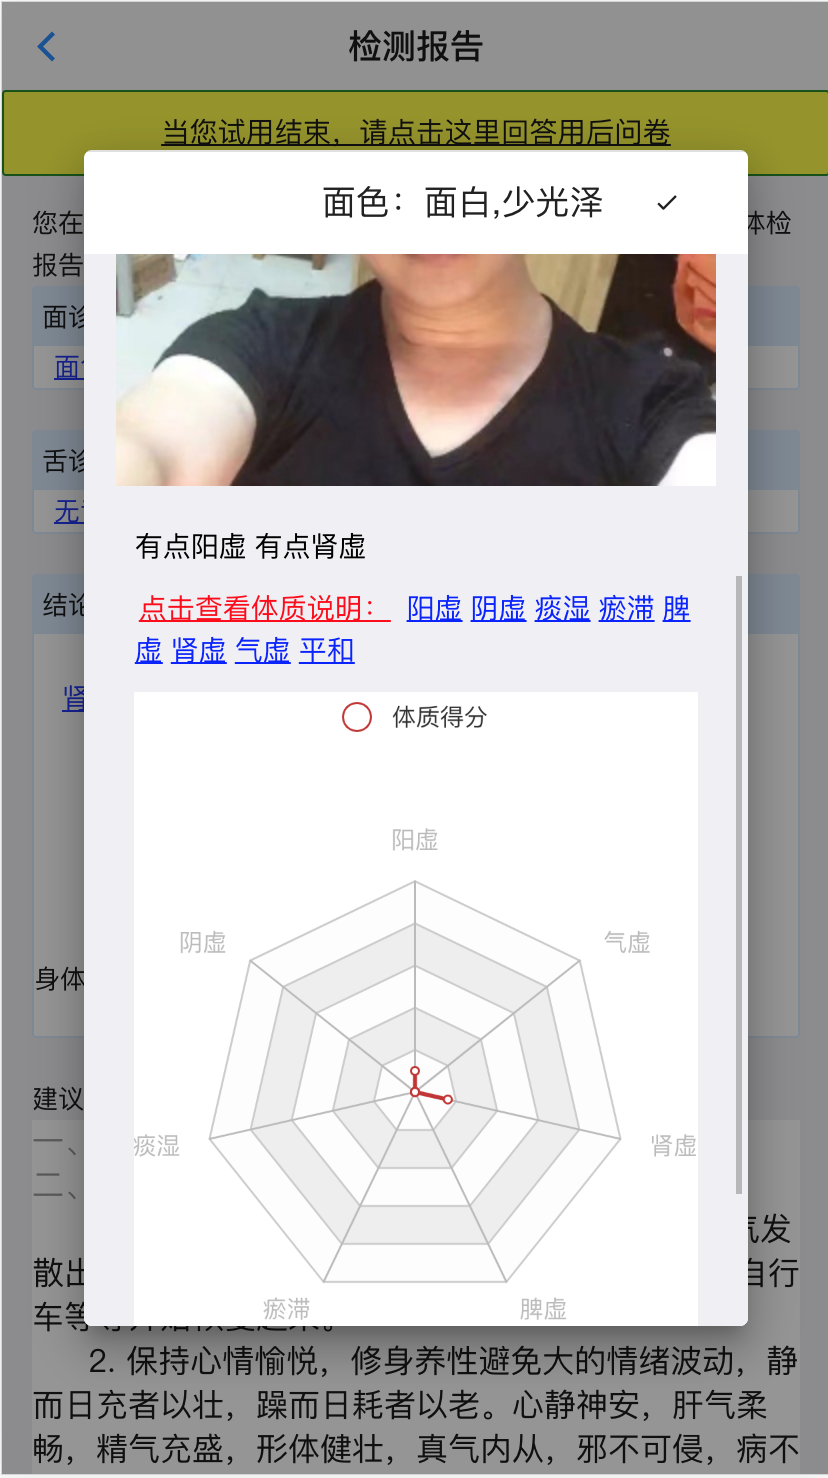
\includegraphics[height=12cm]{images/report4.png}
    \caption{面诊的解释}
    \label{fig:my_label}
\end{figure}

点击体质分数,可以看到当次诊断中,面诊舌诊和用户自己回答的问题,哪些影响到了最后体质的判断。


\begin{figure}
    \centering
    \subfigure[概念的解释]{
        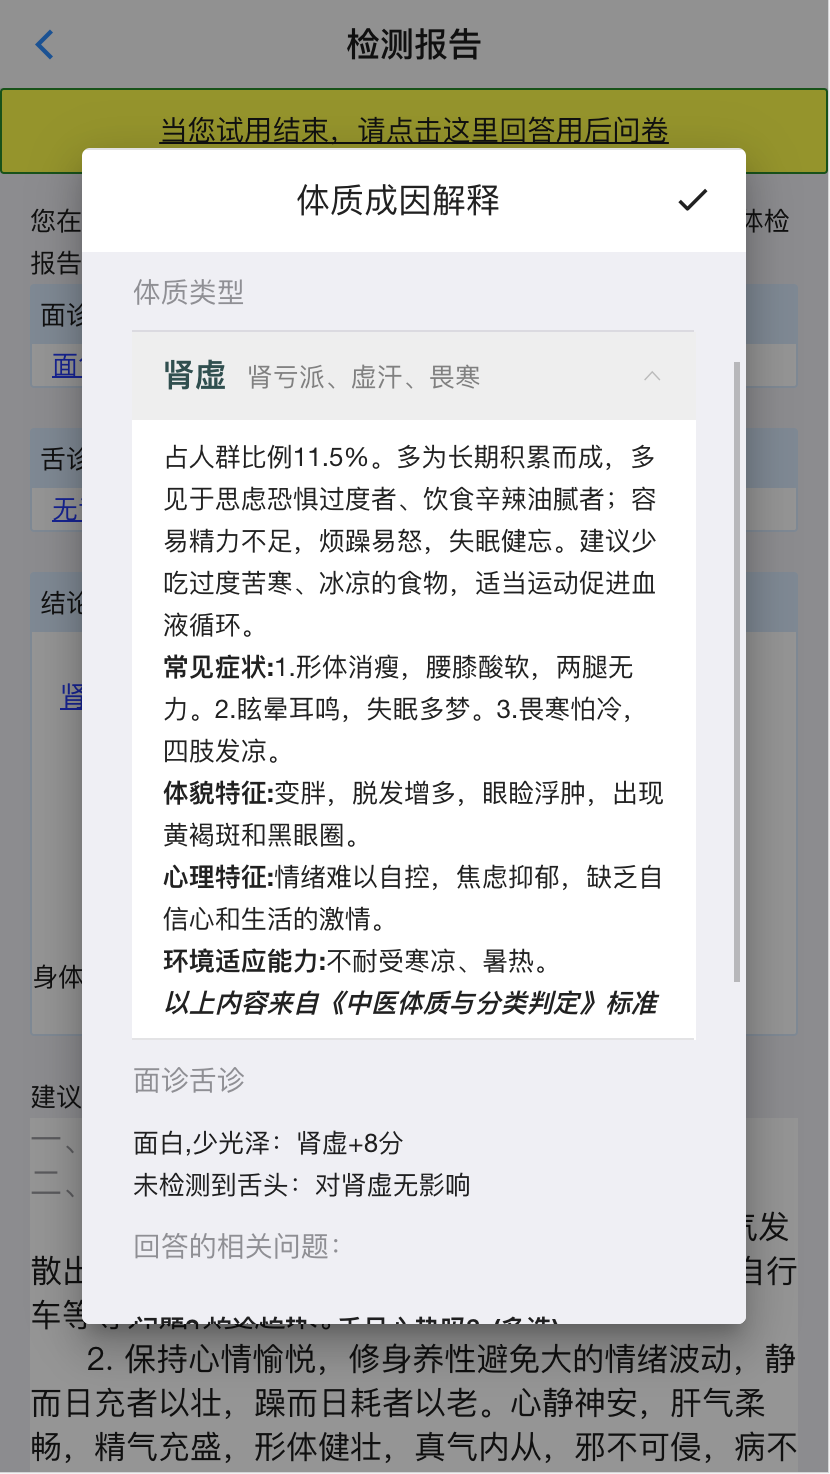
\includegraphics[height=12cm]{images/report5.png}
    }
    \subfigure[体质相关问题]{
        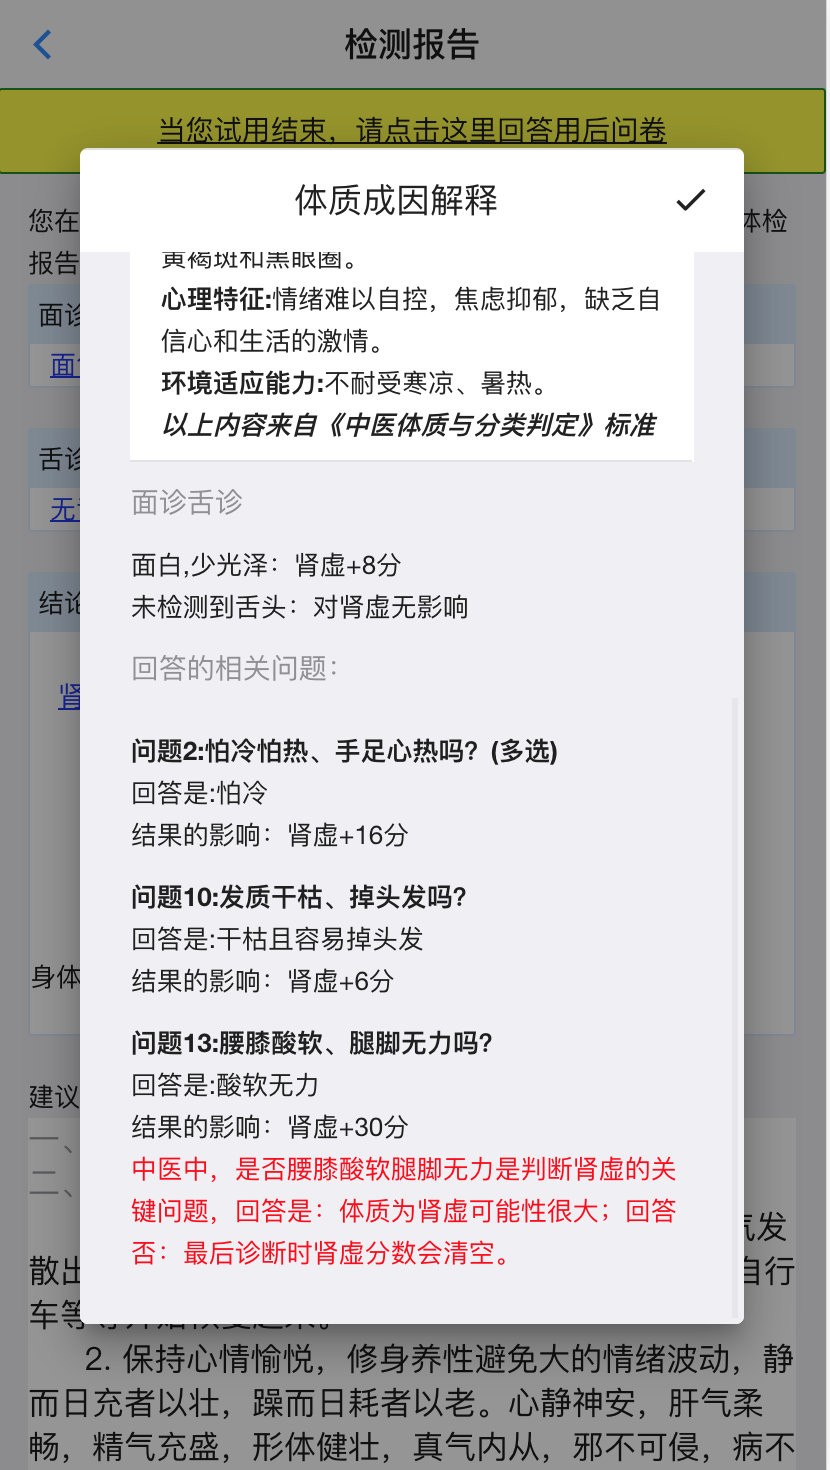
\includegraphics[height=12cm]{images/report6.png}
    }
    \caption{体质的解释}
    \label{fig:report_explain_phy_1}
\end{figure}

